\chapter{Theory (Voorkeur naar eigen informatieve titel)}

Hoofdstuk 2 Theorie: de theorie omvat het theoretisch kader. Daarbij moet gedacht worden aan onderliggende theorie (formules, grafieken, verbanden, verklaringen, aannames e.d.) die nodig is om het onderzoek in goede banen te leiden. Op basis van de theorie kunnen verantwoorde keuzes gemaakt worden (denk aan uitdrukken in meetbare grootheden) en kunnen de resultaten verklaard worden. Het niveau van de theorie is gebaseerd op collegiale toetsing (peer review).

Onderstaand is een kort voorbeeld in het gebruik van LaTeX. Relevante stukken tekst zijn gekopieerd uit een voorgaand verslag. Het gaat hier puur om het gebruik van LaTeX.

Muonen hebben onder andere een toepassing in muon radiografie. Deze techniek gebruikt kosmische straling om holtes in massieve structuren in kaart te brengen. Zo is er op 2 november 2017 een tot op dat moment onbekende kamer in de 'Great Pyramid te Giza ontdekt \cite{PWS}. Voor een toepassing als deze is het van belang dat zowel de massa, snelheid, levensduur en de muonflux op de betreffende plek zo nauwkeurig mogelijk bekend zijn. \\

Tijdens het onderzoek behorende bij dit verslag zal de muonlevensduur in rust onderzocht worden. De onderzoeksvraag luidt als volgt.
\begin{itemize}
	\item Meet de levensduur van een muon en bepaal de bijbehorende onnauwkeurigheid. Vergelijk je waarde met de literatuur.
\end{itemize}

Muonen zijn elementaire deeltjes die ontstaan ten gevolge van kosmische straling die de aardatmosfeer binnenkomt in de vorm van protonen \cite{bbnikhef}. De vervalreeks tengevolge van deze binnenkomende protonen is weergegeven in Figuur \ref{fig:air_shower}. De muonen die hierbij vrijkomen ontstaan op ongeveer 15 km hoogte  \cite{air_shower}.
\begin{figure}[!htbp]
\begin{center}
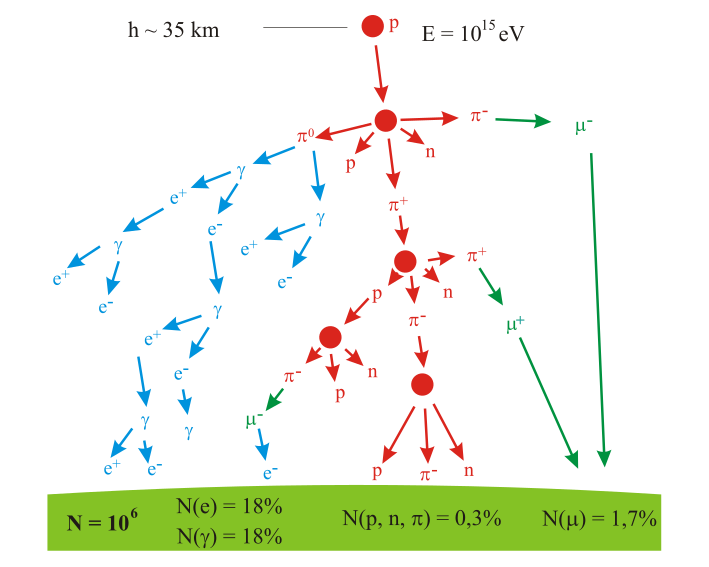
\includegraphics[width=\textwidth]{figuren/air_shower.png}
\end{center}
\caption{De vervalreeks van een proton die met lucht moleculen botst \cite{air_shower}.}\label{fig:air_shower}
\end{figure}

\begin{figure}[!htbp]
\begin{center}
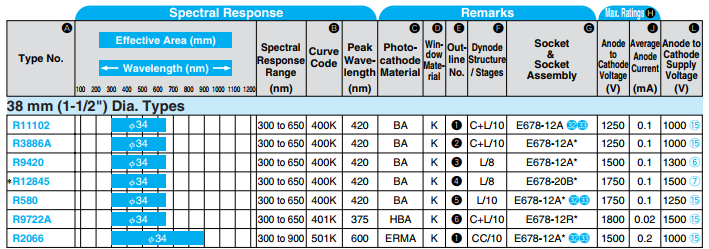
\includegraphics[width=\textwidth]{figuren/PMTspecs}
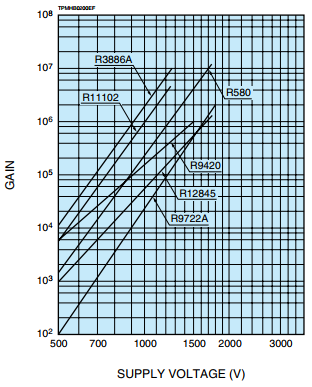
\includegraphics[width=\textwidth]{figuren/PMTgain}
\end{center}
\caption{De specificaties van de Hamatsu R580 PMT's \cite{pmtmanual}.}\label{fig:pmtspecs}
\end{figure}

\begin{equation}
	\Phi_{R580} = 21,7 \quad \mathrm{[muonen/s]}
\end{equation}

Uit bron \cite{masterthesis} blijkt dat de volgende instellingen

\begin{equation}
		1200 \leq V_{PMT} \geq 1600 \quad \mathrm{[V]}
\end{equation}
\begin{equation}
	20 \leq V_{Threshold} \geq 30 \quad \mathrm{[mV]}
\end{equation}

dienen te leiden tot onderstaande resultaten:

\begin{equation}
	\Phi_{R580} = 21,7 \quad \mathrm{[muonen/s]}
\end{equation}
\begin{equation}
	\tau_{\mu} =   2,00 \times 10^{-6}\quad \mathrm{[s]}
\end{equation}
\begin{equation}
	\overline{v}_{\mu} = (0,99 \pm 0,017) c \quad \mathrm{[m/s]}
\end{equation}

Hierbij is $V_{PMT}$ het potentiaalverschil tussen de anode en de cathode van de PMT. De drempelspanning $V_{Threshold}$ is de minimum spanning die vereist is om een binnenkomende puls te registreren als puls afkomstig van een muon. De levensduur $\tau_{\mu}$ is de levensduur van het muon welke in het verleden met hetzelfde type opstelling gemeten is \cite{masterthesis}. De gemiddelde snelheid $\overline{v}_{\mu}$ is de al eerder gemeten gemiddelde snelheid waarmee muonen zich voortbewegen. Deze is in overeenstemming met de literatuur waarde van 0,99c \cite{masterthesis}.

Bij de uitvoering van dit onderzoek is onderstaand materiaal vereist.

\begin{itemize}
	\item Twee muonbalken
	\item Twee BMC-kabels
	\item Twee kabels voor de spanning van de PMT's
	\item Muonlab III kastje
	\item USB-kabel
	\item Computer met LabVIEW en de Muonlab III VI
\end{itemize}

Middels de 'cftool' add-on voor matlab is er tot de onderstaande resultaten gekomen voor de fit.
\begin{equation}
N_0 = 618 \quad \tau = 2,09\cdot10^{-6} \quad c = -8,24 \label{eq:lifetime_fit}
\end{equation}

Tabel gemaakt met: https://www.tablesgenerator.com/. Merk op dat aan de tabellen wat code aangepast moet worden.
% Please add the following required packages to your document preamble:
% \usepackage{graphicx}
\begin{table}[h!]
\centering
\caption{De levensduur $\tau$ welke gehaald is uit de lifetime metingen. De R$^2$ behoort bij de fit gedaan volgens Vergelijking \ref{eq:lifetime_fit}.}
\label{tab:levensduur}
\begin{adjustbox}{max width=\textwidth}
\begin{tabular}{|c|c|c|}
\hline
\textbf{Sample}  & \textbf{Levensduur $\tau$} & \textbf{R$^2$}   \\ \hline
\textbf{{[}-{]}} & \textbf{{[}$\mu$s{]}}      & \textbf{{[}-{]}} \\ \hline
6                & 2.245                      & 0,9968           \\ \hline
8                & 2,660                      & 0,9641           \\ \hline
9                & 1,443                      & 0,9956           \\ \hline
10               & 2,137                      & 0,9997           \\ \hline
\end{tabular}%
\end{adjustbox}
\end{table}